
\chapter{Colloid diffusion in glass capillary tubes}
\label{ch3_extras}

\section{Introduction}
Understanding the outliers in diffusive processes is the key to describing many important phenomena, such as biological processes dependent on the interactions between strands of DNA, patient zero spreading a virus to a new area in a pandemic, many chemical processes, and how microscopic price fluctuations relate to long-term macroscopic trends in the stock market~\cite{zhang_first-passage_2016, hufnagel_forecast_2004, redner_8_2001, liu_anchoring_2017}. How do we predict the behavior of these furthest or fastest particles? In diffusive environments, where many particles spread outward from their originating source, we can use Einstein’s treatment of diffusion to describe the bulk behavior of the particles~ \cite{einstein_uber_1905, von_smoluchowski_zur_1906}. Einstein described diffusion as particles undergoing independent random walks, but the independent nature of these walks ignores the effect the shared environment has on the particles. As a result, when analyzing the system as a whole, the distributions of outlier particle locations and first passage times should differ from those predicted by Einstein’s theory. We have designed an experimental system to measure the first passage times of micron-sized silica beads suspended in water travelling in narrow, quasi-1D glass capillary tubes to measure these extreme value statistics and demonstrate this difference.
 
% \begin{figure}[hb]
% \begin{center}
% \includegraphics[width=0.9\columnwidth]{Figures/model_both_sidebyside.png}
% \caption{\label{fig:1D_BC} 1D visualization of the Einstein and Barraquand-Corwin models, where the red and blue colors indicate the direction of each bias - right and left, respectively - and the color intensity indicates the strength of the bias; for example, a dark red square indicates a strong bias to the right for the particles inhabiting that square. White squares have an equal bias in each direction. Time increases from the bottom of the image toward the top.}
% \end{center}
% \end{figure}

% \begin{figure*}[htp]
% \begin{center}
% \includegraphics[width=0.9\columnwidth]{Figures/TriangleGrowth-01.png}
% \caption{\label{fig:comparison} Einstein and Barraquand-Corwin diffusion models. Einstein's diffusion model has an equal bias in each direction, and the particles diffuse accordingly. For the Barraquand-Corwin model, the red and blue colors and color intensity indicate the direction and strength of the bias as in Figure \ref{fig:1D_BC}. Time increases from the bottom of the image toward the top. There is a noticeable difference in how the outlier particles for each model spread in the same amount of time.}
% \end{center}
% \end{figure*}

\section{Background}
\acg{[determine how much of this is necessary given Chapter \ref{1Drandom}'s existence - this is mostly from comp exam and needs rewritten]}

While Einstein's traditional independent random walk model describes the average behavior well in many systems, there are areas where this theory and its predictions are known to fail. Some systems, such as Brownian motion in supercooled liquids and close to jamming, flow and drainage, friction, and turbulence, where probability distributions display exponential tails and other non-Gaussian characteristics~\cite{wang_when_2012, metzler_brownian_2019}. Additionally, Einstein’s theory fails to describe the full dynamics of active matter, where particles inject energy into the environment; such is the case with self-propelled particles exhibiting loopy trajectories and active particles capable of absorbing and dissipating energy~\cite{kanazawa_loopy_2020, ramaswamy_mechanics_2010}. The difference between systems with these dynamic particles and those well characterized by independent random walks is well described by contrasting these probability distributions, especially in the extremes.

\acg{[I need to revisit this claim] Studying and modelling first-passage particle behavior has been done, but this work often neglects systems where particle motion is correlated}~ \cite{grebenkov_exact_2020}. Guillaume Barraquand and Ivan Corwin developed a theoretical model for diffusion that explicitly includes correlations resulting from the shared background environment by modelling diffusion as a random walk with transition probabilities drawn from the beta distribution~ \cite{barraquand_random-walk_2017}. The Barraquand-Corwin model predicts the behavior of the maximum of a large number of ``walkers’’ and reveals a connection to the Kardar-Parisi-Zhang universality class with a related phase transition~ \cite{barraquand_random-walk_2017, barraquand_moderate_2020, le_doussal_diffusion_2017, kardar_dynamic_1986}. In times comparable to $log\left(N\right)$, there is a connection between the large deviations of transition probabilities in a random walk in random environment (RWRE) and the Kardar-Parisi-Zhang (KPZ) universality class's Tracy-Widom GUE distribution [cite lots of papers, see Hass paper]. In  the $log\left(N\right)^{2}$ time frame, the Tracy-Widom GUE distribution is replaced by that of the KPZ equation [also cite things from Hass paper, and Hass paper]. Numerical simulations from Chapter \ref{1Drandom} confirmed these scalings in these regimes.

Further work done by Hass et al\acg{[cite the FPT paper(s)]} describes how the first passage time scales with particle number.

%

\begin{figure*}[htp]
\begin{center}
\includegraphics[width=0.35\columnwidth]{Figures/microscope_centrifuge.png}
\caption{\label{fig:CADrender} Experimental setup}
\end{center}
\end{figure*}

\acg{[first draft of everything below this point]}

\section{Experimental design}

To measure EFPTs in a physical system of colloids, we developed a microscope-centirfuge system, shown in Figure \ref{fig:CADrender}. The centrifuge consists of a flat rotor plate, which holds 16 samples and inside gaps for imaging, fixed to A DC motor (McMaster-Carr 59835K62) via screw-clamp bushing (McMaster-Carr 5926K16). Angular position of the plate is encoded by 16 bits via incremental optical rotary motion encoder (McMaster-Carr, 9749T2). By also tracking angular velocity via tachometer, we get down to 3mm positioning precision. A 12V sealed linear solenoid (McMaster-Carr 69905K173) acts as a brake to help lock in the final position. A custom machined aluminum base plate and support arm bolted to the optics table provide stability. A microcontroller (Arduino Mega) controls an external analog servo system, using a total of 19 digital pins -- 1 pin each to trigger the brake, turn servo mode on/off, and run the centrifuge at full speed outside of servo mode; in servo mode, 16 digital pins write a 16-bit location. The top speed of the centrifuge is currently unknown, but likely exceeds 1000 RPM. \acg{(mayhaps I should try to cover the holes and measure this again)}

An upright fixed stage microscope (Nikon ECLIPSE FN1) with either 4x or 10x objective (it is switchable, 4x gets more FOV but idk what it does about depth of field) with a camera (Teledyne Blackfly S USB3) is used to image silica microspheres (Cospheric monodisperse silica microspheres, 1.18 $\mu$m diameter) suspended in deionized (maybe bad?) water and sonicated to disperse aggregates, at a concentration of 1\% by volume. We coat the interior of 100mm long rectantular capillary tubes (Vitrocom VitroTubes™ 5003, 5004), 0.3mm/0.4mm wide and 0.03mm/0.04mm tall, with bovine serum albumin (BSA), flushing out the excess with pressurized air. This interior coating will help prevent silica microspheres from adhering to the capillary walls \acg{(cite someone that says this maybe?)}. We then fill the tubes with the silica suspensions, break off any air pockets, and seal the ends with capillary wax (Sigillum wax sealant). We dip the now-sealed ends in cyanoacrylate glue to provide a strong seal for when the centrifuge spins the samples down at high angular acceleration. The capillary surface is then cleaned with isopropyl alcohol and lens paper.

This process is repeated for 16 capillary tubes, with each tube placed into its own channel on the centrifuge plate. Care is taken to ensure the capillaries are as level/flat as possible to prevent gravity-driven flow in the solutions. Melted paraffin wax is carefully poured onto the non-imaging parts of each capillary, which, once cooled, adheres the capillaries in place in the channel. Once all 16 capillaries have been adhered, the centrifuge process may begin.

A MATLAB script controls both the Arduino for centrifuge operation and the camera for imaging. Upon starting the script, the Arduino pins and camera are initialized, and directories based on the datetime are created for data storage. The centrifuge enters run mode for a preset amount of time, where it spins at the highest attainable speed. After the time runs out, the centrifuge slows down, and the 16 position pins send it to the "16th" capillary location. The centrifuge then carefully pans through each location, collecting an initial "reference" image of each of the 16 capillaries. The script then enters time-lapse mode, where, based on a preset time gap, the centrifuge pans through each location and collects a new frame for each capillary. Each frame is stabilized relative to its initial "reference" frame and writing this corrected frame to an image file that capillary's image directory. After cycling through each capillary, the system pauses for the allotted time, then cycles through to collect and stabilize frames again. This repeats indefinitely, or until the user ends this sequence. The final parts of the script close the camera and clear all variables for the next collection.
 
\begin{figure*}[htp]
\begin{center}
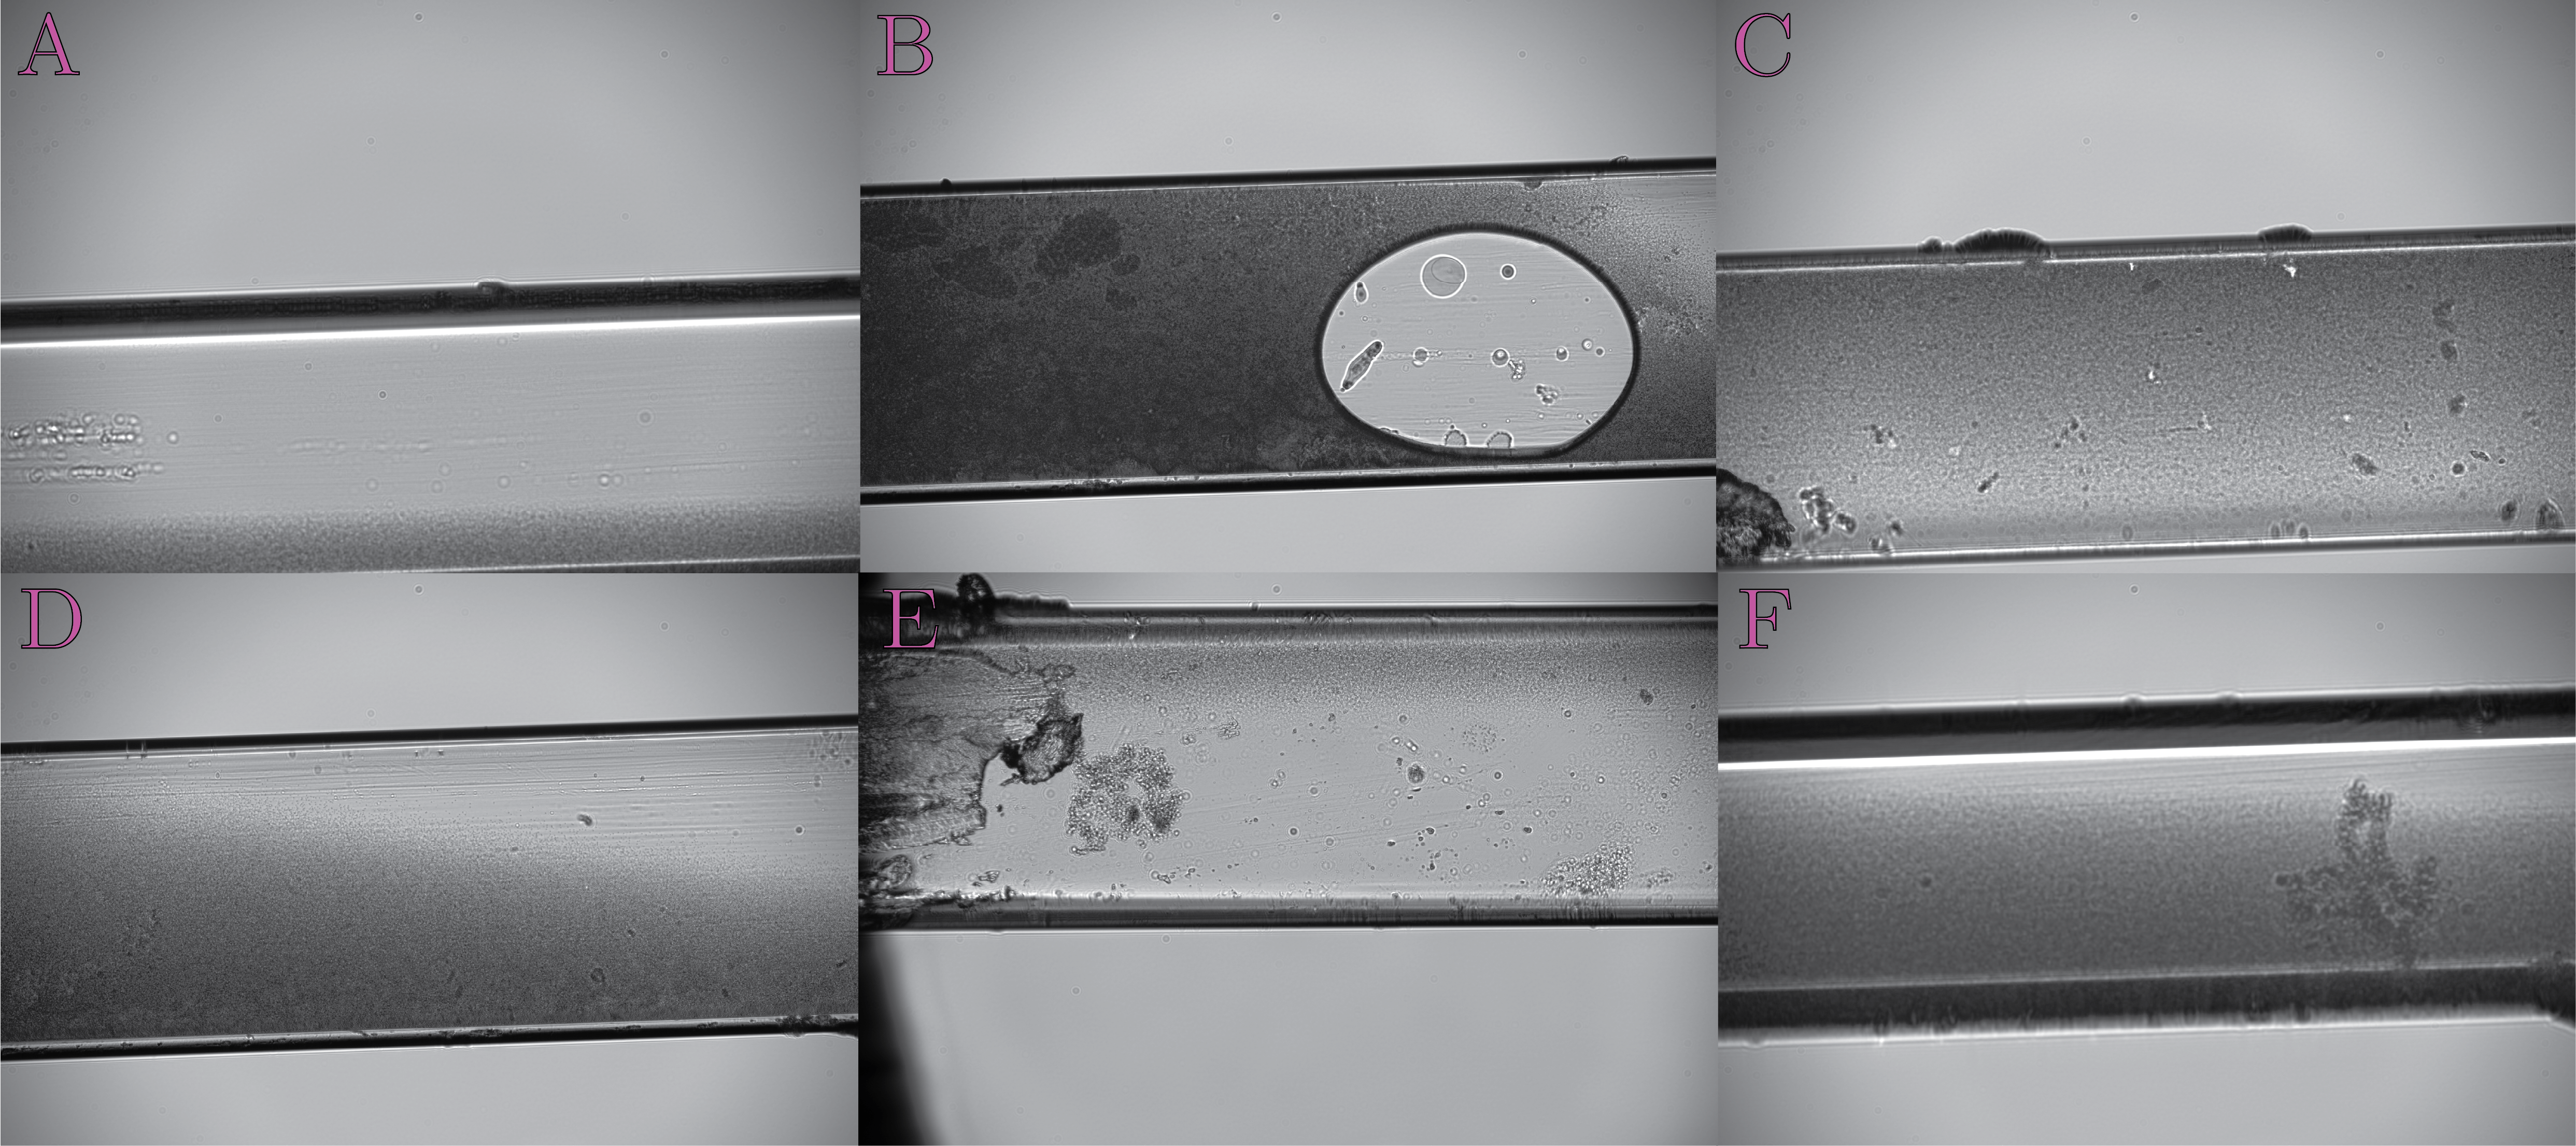
\includegraphics[width=0.9\columnwidth]{Figures/capillaries.png}
\caption{\label{fig:caps} Examples of imaged capillaries}
\end{center}
\end{figure*}

\section{Results}
Preliminary results show that it is possible to centrifuge down samples in capillary tubes such that the majority of the colloids end up on the outer end. By removing air bubbles beforehand, and coating the tubes with bovine serum albumin, we minimize bulk flow and colloids sticking to the glass. Image stabilization removes discrepancies in the servo positioning and enables tracking of particles using packages such as Trackpy. Blah blah Figure \ref{fig:caps} shows issues. Would be nice to run tracking on sequence but idk if I'll get to that or not.

\section{Discussion/Conclusion}
While we have good descriptions for regular diffusion and average particles, and have been able to do so for a long time now, we have only recently been able to understand the extremes and characterize their statistical behavior. We have designed, built, and tested an experimental setup that allows us to measure first passage times in colloid diffusion. Further refinement is needed to make complete measurements, but preliminary results are promising, and the concept is sound.
%%

%\bibliography{scaling}% Produces the bibliography via BibTeX.


%\end{document}
%
% ****** End of file aipsamp.tex ******

